A \textit{landing page} do projeto foi desenvolvida em \textit{HTML}, responsável pela estrutura do conteúdo, \textit{CSS}, utilizado para o estilo visual, e \textit{JavaScript}, empregado na implementação da interatividade e do dinamismo da navegação. O sistema de rastreamento ocular foi implementado em JavaScript, utilizando a biblioteca \textit{WebGazer.js}, que contém um modelo capaz de se autocalibrar ao observar a interação dos visitantes com a página, treinando um mapeamento entre as características do olhar e as posições na tela \cite{papoutsaki2016webgazer}. O tratamento das coordenadas oculares recebidas do \textit{frontend} foi realizado em JavaScript, com o uso do \textit{Node.js} e do \textit{Socket.IO}, possibilitando a comunicação em tempo real com o frontend, uma vez que depende das coordenadas enviadas por ele. Essa parte do \textit{backend} é responsável por analisar as métricas TDC (acertos e erros), dados que serão utilizados para compor o feedback individual de cada usuário. No backend, a biblioteca serialport gerencia a comunicação serial pela porta COM \textit{(Windows)}, enviando comandos ao dispositivo IoT e recebendo eventos, integrados ao frontend em tempo real via Socket.IO. Por fim, o jogo \textit{web} foi desenvolvido em \textit{TypeScript}, utilizando o \textit{framework} \textit{Next.js}, o que proporcionou um código mais robusto, organizado e uma experiência de uso moderna e fluida.

A metodologia fundamenta-se na aplicação adaptada do TDC. A principal diferença do presente trabalho está na integração do teste com o rastreamento ocular em tempo real, permitindo a coleta de dados visuais complementares durante a execução das tarefas.

O experimento é estruturado como um jogo digital de temática espacial, composto por três fases com níveis crescentes de dificuldade. A mecânica de jogo foi desenhada para simular os princípios do TDC, promovendo a exposição contínua a estímulos visuais por períodos prolongados e exigindo respostas rápidas e consistentes por parte do participante. 

Durante toda a experiência, o rastreamento ocular é realizado em segundo plano, utilizando a biblioteca WebGazer.js para capturar os pontos de fixação visual do usuário por meio da \textit{webcam}. Para garantir a precisão da predição do olhar, a WebGazer.js utiliza uma arquitetura que combina diferentes técnicas de Aprendizado de Máquina. Inicialmente, o TensorFlow FaceMesh é mobilizado para a detecção precisa e em tempo real da face e, especificamente, dos pontos de referência da região ocular. O modelo de predição propriamente dito é baseado na Regressão Ridge, que é uma variação da regressão linear. A principal função desta técnica é atuar como um mecanismo de regularização, que, simplificadamente, evita o superajustamento \textit{(overfitting)} do modelo. Isso significa que ela impede que o modelo fique muito focado nos dados de treinamento, o que faria com que ele errasse ao lidar com novos usuários. A Regressão Ridge faz isso aliviando a influência dos parâmetros de maior valor no aprendizado. O resultado é um modelo mais robusto e generalizável, capaz de realizar o mapeamento entre a imagem dos olhos e as coordenadas da tela de forma confiável para diferentes participantes. Finalmente, no pós-processamento, as predições de olhar bruto são submetidas ao Filtro de Kalman, um algoritmo recursivo que suaviza os dados, aumentando a fluidez e a estabilidade da predição ao estimar o próximo ponto de fixação com base na observação anterior \cite{WebGazerDoc}.É importante notar que todos os componentes algorítmicos, incluindo FaceMesh, Regressão Ridge e Filtro de Kalman, são nativos da biblioteca WebGazer.js e foram empregados em sua configuração padrão, sem modificações.

Os dados de fixação visual coletados permitem identificar padrões de atenção ou desatenção, que são contrastados com nossa base de dados em cada etapa da atividade. Em paralelo à coleta desses dados, todas as fases do experimento são configuradas para potencializar a sobrecarga sensorial e dificultar a concentração do participante. Para tal, utilizam-se música de fundo — cuja intensidade e ritmo são ajustados conforme o nível de dificuldade — e a imposição de um tempo máximo definido, elementos que, em conjunto, intensificam o estresse cognitivo e a exigência da tarefa.

Após o realizar \textit{login}, o participante é direcionado para a página de instruções, onde são apresentadas a sequência de como calibrar o olhar para poder prosseguir para o jogo. Antes de cada fase, existem as instruções da mesma. Em seguida, o usuário inicia a primeira etapa do teste. 

\begin{figure}[H]
    \centering
    \caption{Primeira fase}%
    \label{fig:primeira-fase}
    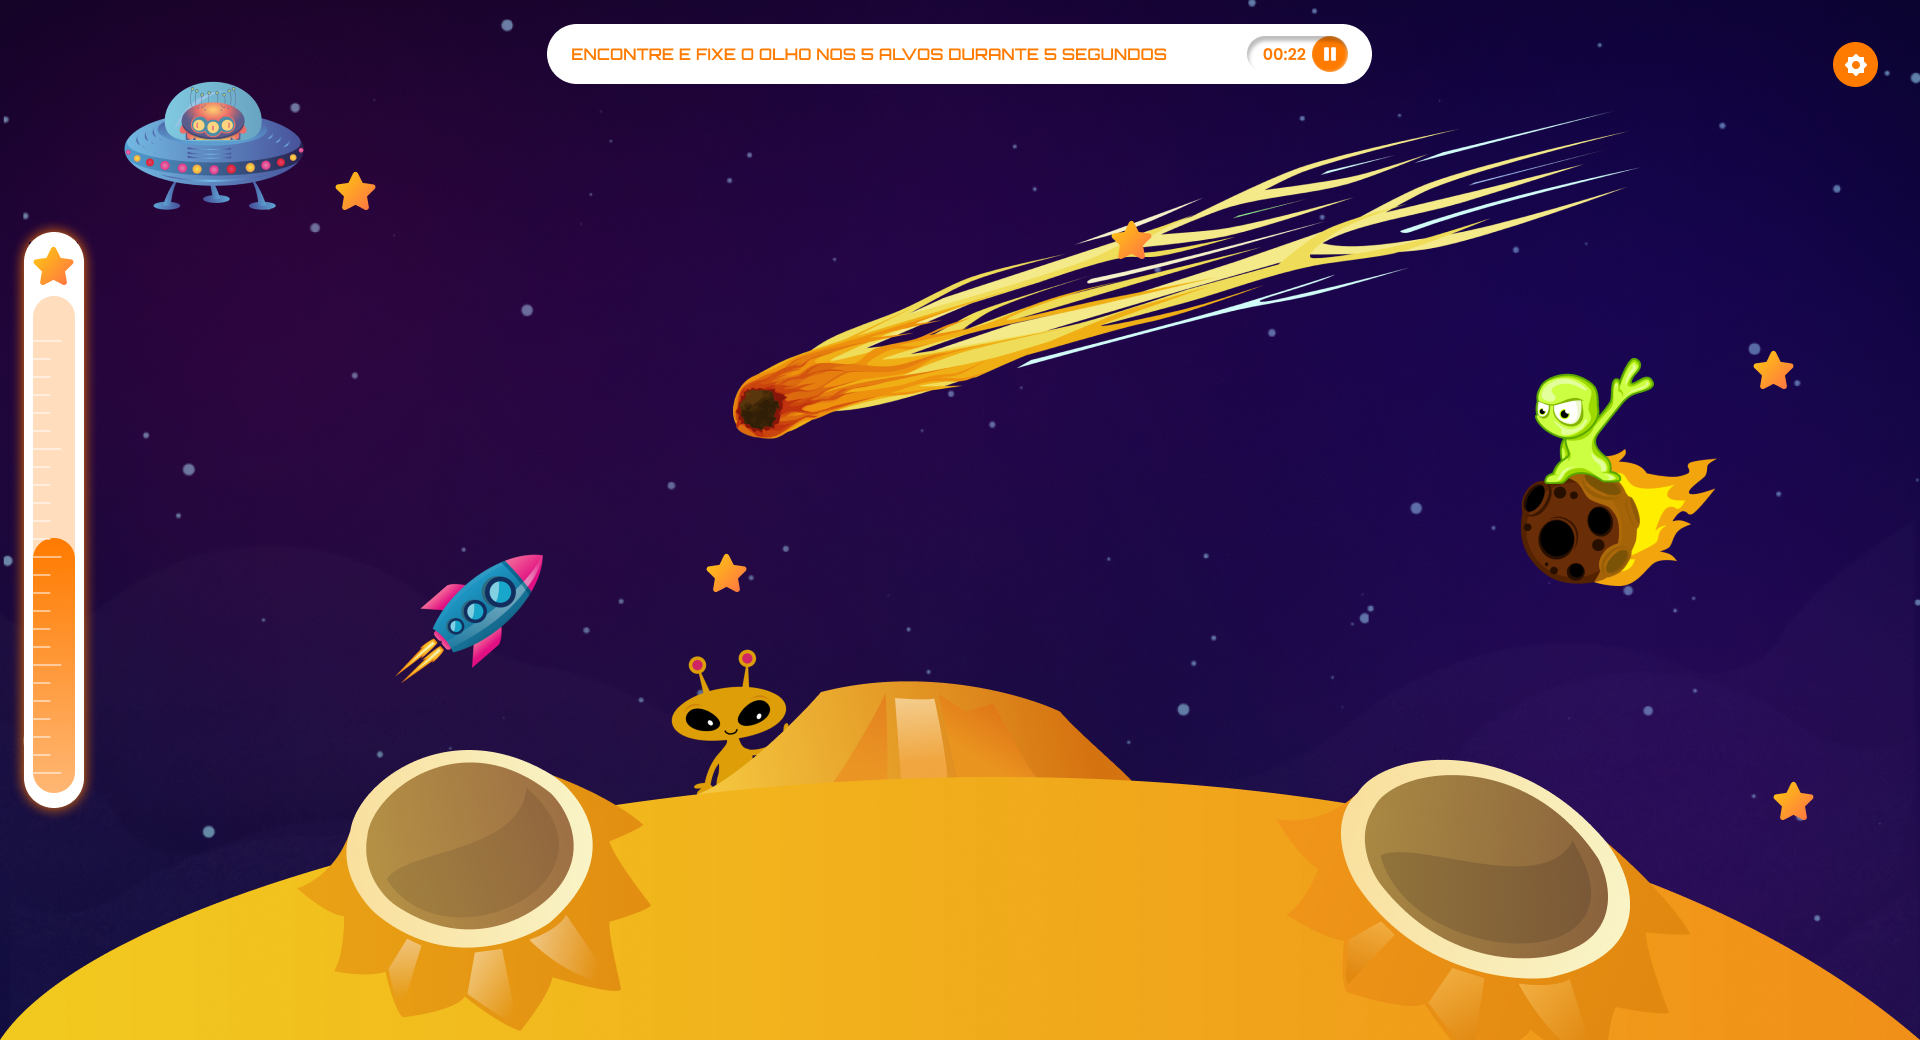
\includegraphics[width=\textwidth]{primeira-fase.png}%
    \SourceOrNote{Autoria Própria (2025)}
\end{figure}

Na primeira fase, o participante deve fixar o olhar por cinco segundos em cinco alvos estáticos,
representados por estrelas, enquanto elementos animados surgem ao redor. Após os 5 segundos,
cada estrela desaparece da tela. A música de fundo nesta etapa apresenta um ritmo moderado. O tempo total da fase é de 1 minuto. O
objetivo é avaliar a capacidade de manter a atenção em um ponto fixo durante um tempo determinado, ignorando estímulos visuais e auditivos periféricos.

Ao iniciar a fase, uma conexão via WebSocket é aberta entre o cliente (front-end) e o servidor (back-end). O servidor reconhece o cliente conectado, que envia as coordenadas das estrelas para o endpoint $\texttt{/iniciar\_experimento\_com\_config}$. O eye tracking é iniciado, e o cliente começa a enviar as coordenadas dos olhos a cada 1 segundo para $\texttt{/gaze\_data}$. O servidor, por sua vez, escolhe uma dentre as cinco estrelas para ser o alvo atual, e o cliente escuta através de $\texttt{/fase\_iniciada}$, pois este é responsável por deixar a estrela em destaque e, ao mesmo tempo, continua transmitindo as coordenadas dos olhos.Em seguida, o servidor conta até 10 segundos para que o usuário olhe fixadamente para a estrela por, no mínimo, 5 segundos. Se o usuário olhar por 5 segundos ou se o tempo de 10 segundos se esgotar, o servidor comunica que a fase terminou através de $\texttt{/fase\_atual\_finalizada}$. O cliente, então, deleta a estrela que antes estava em destaque, e o servidor escolhe uma nova estrela para ser o alvo atual. Esse processo se repete até que todas as estrelas sejam apresentadas.Ao final da fase, o servidor é responsável por salvar o objeto $\texttt{historico\_olhar\_fase1}$ no banco de dados, que contém o estado do olhar (sendo $\texttt{1}$ para olhando e $\texttt{0}$ para desviando), um timestamp e o índice do alvo atual. Além desse objeto, o $\texttt{resultado\_alvos\_fase1}$ também é salvo, contendo o índice do alvo, se terminou por sucesso ou por tempo esgotado, o tempo de início do alvo e o tempo de término do alvo.Ao ter esses dados salvos, o servidor calcula as métricas TDC da Fase 1, que são: número de acertos (olhou por 5 segundos), número de erros de omissão (demorou 10 segundos ou mais para começar a olhar), erros de comissão (começou a focar antes de 10 segundos, mas não manteve o foco por 5 segundos), o tempo médio de reação (tempo que levou para olhar para o alvo) e o desvio padrão. Essas métricas são enviadas ao cliente através de $\texttt{/fase\_concluida}$, para que o usuário visualize seu desempenho na fase, conforme ilustrado na Figura \ref{fig:fim-fase1-fase3}.

\begin{figure}[H]
    \centering
    \caption{Resultados da fase 1}%
    \label{fig:fim-fase1-fase3}
    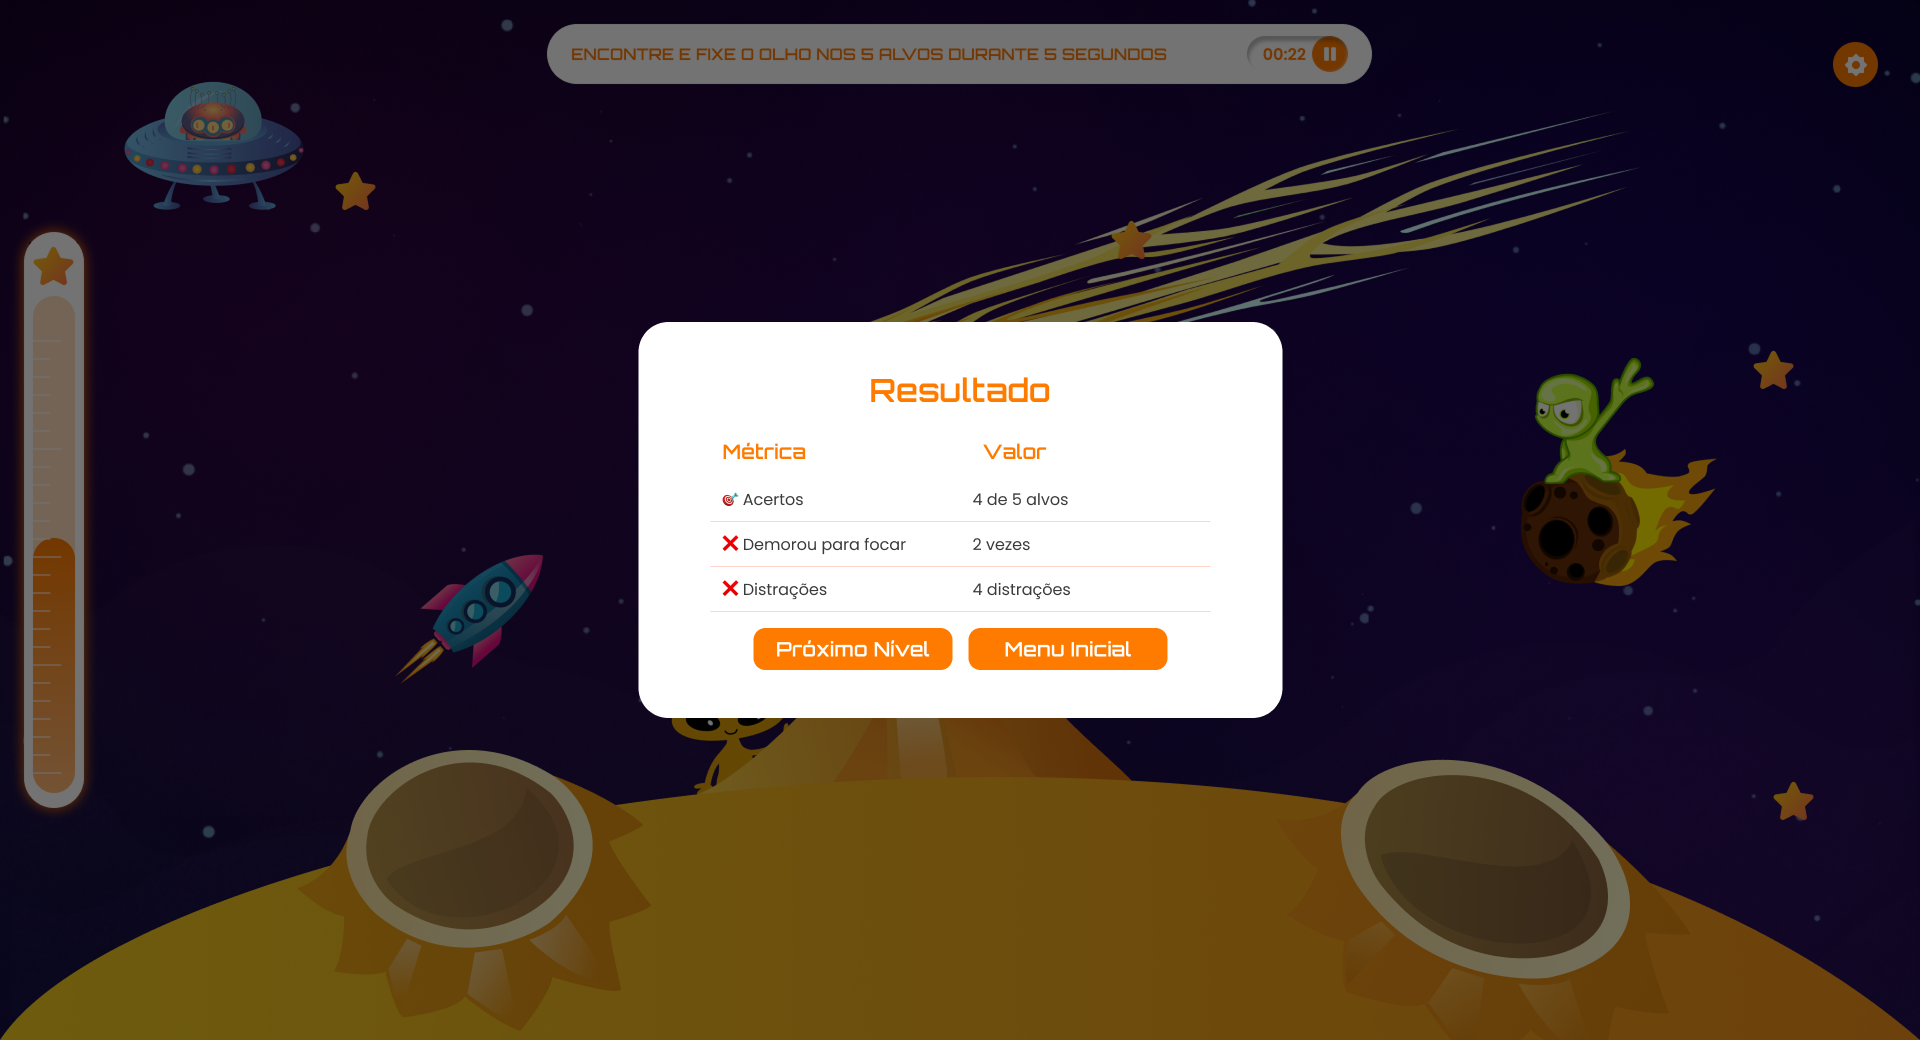
\includegraphics[width=\textwidth]{fim-fase1-fase3.png}%
    \SourceOrNote{Autoria Própria (2025)}
\end{figure}

\begin{figure}[H]
    \centering
    \caption{Segunda fase}%
    \label{fig:segunda-fase}
    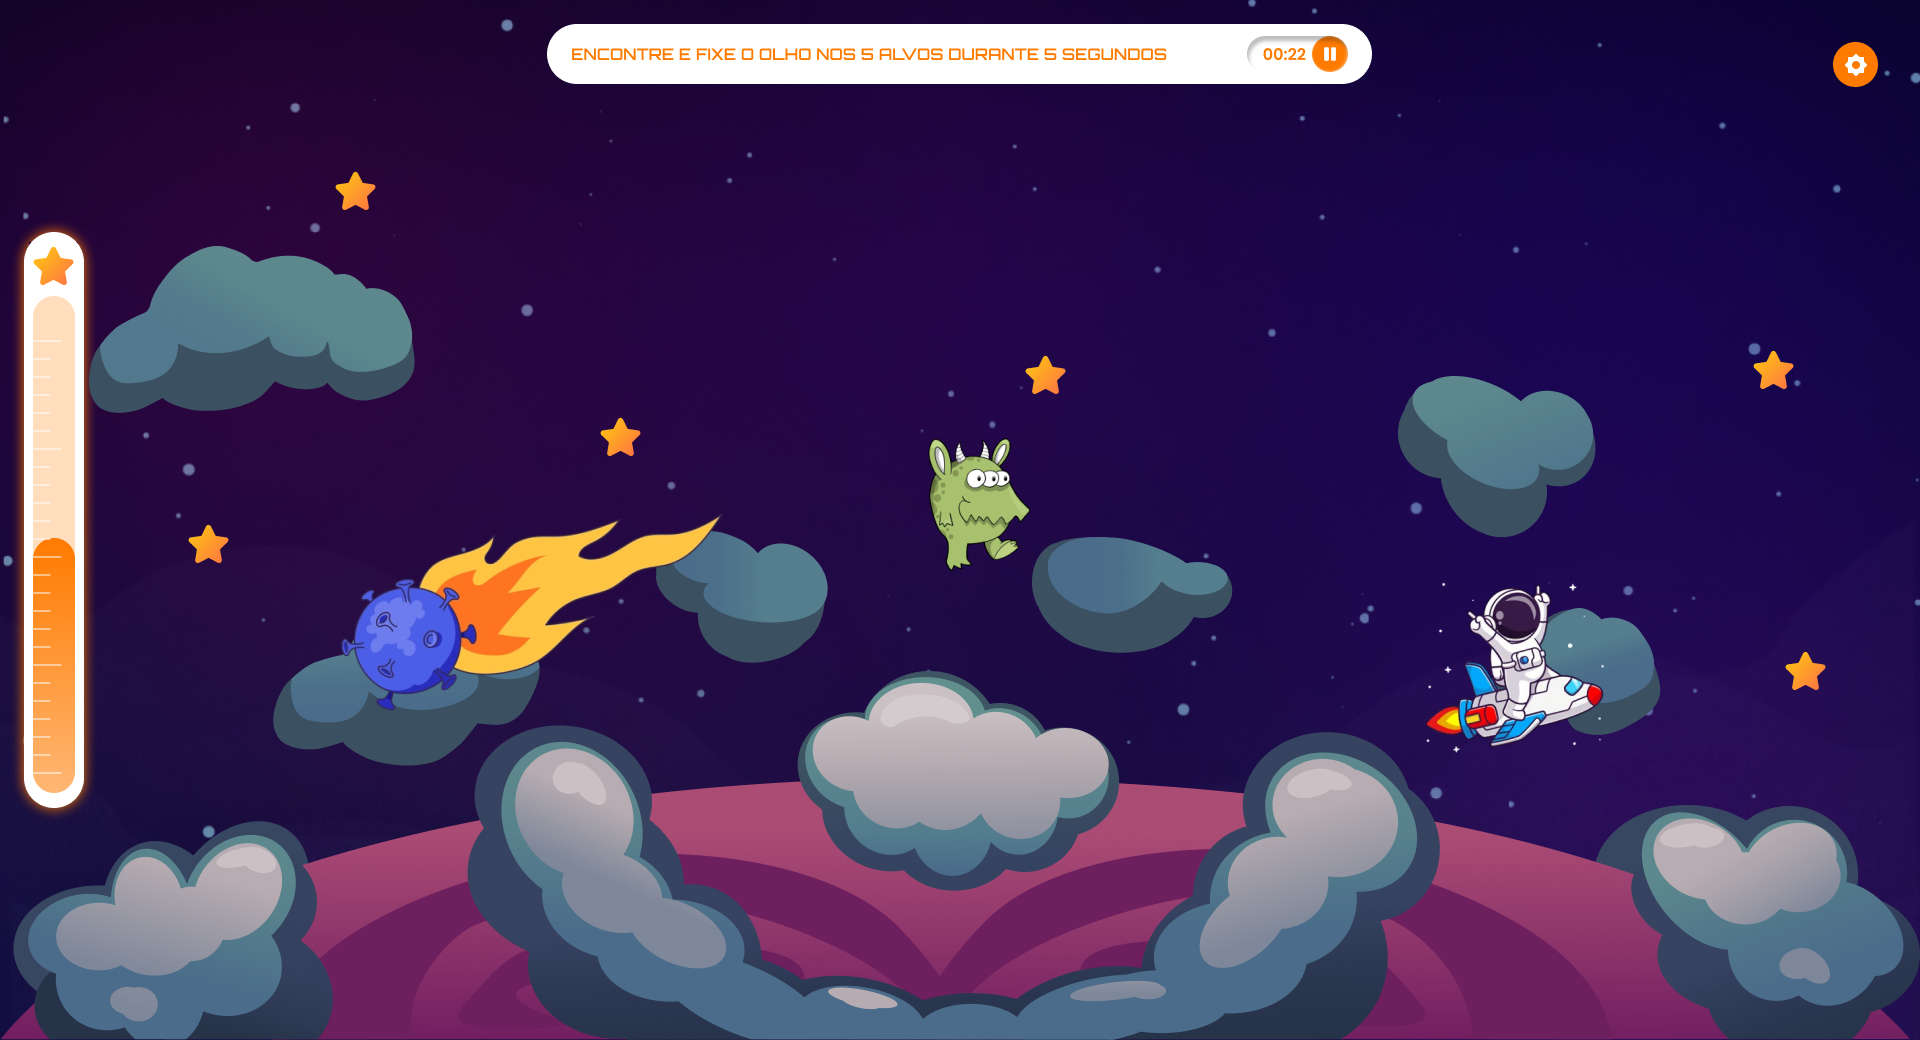
\includegraphics[width=\textwidth]{segunda-fase.png}%
    \SourceOrNote{Autoria Própria (2025)}
\end{figure}

Na segunda fase, o participante deve manter o foco em cinco estrelas estáticas, que brilham alternadamente (estímulo primário). Simultaneamente, três planetas em movimento transitam pela tela, atuando como distratores (estímulos secundários) cuja presença não é mencionada nas instruções. A fase 2 é composta por duas rodadas iguais de 15 segundos cada, onde apenas os planetas que transitam pela tela são alterados. Ao término de cada rodada, o participante é submetido a um teste de reconhecimento: sete opções de planetas são apresentadas, sendo que apenas três transitaram na tela. O participante deve indicar, por meio de botões IoT, quais planetas foram reconhecidos durante o trânsito. O reconhecimento correto de planetas efetivamente exibidos é contabilizado como acerto, enquanto a seleção de planetas não exibidos configura erro. Dessa forma, passadas as duas rodadas, ou seja, ao final da fase, são exibidos: quantidade de acertos, planetas vistos e planetas ignorados. Essa etapa avalia simultaneamente o desempenho na tarefa principal e a detecção incidental de estímulos periféricos. A interpretação do reconhecimento de estímulos secundários como indicador positivo ou negativo será definida após validação com grupos de referência (crianças com e sem TDAH), considerando duas hipóteses alternativas: (1) maior detecção incidental pode refletir dificuldade de inibição de distratores e associar-se ao TDA; (2) menor detecção, decorrente de foco mais exclusivo na tarefa principal, pode estar mais associada ao TDA. A trilha sonora, mais intensa e acelerada nesta fase, eleva a carga cognitiva e permite observar o impacto de múltiplos estímulos simultâneos na manutenção da atenção.

No início da fase 2, uma conexão via WebSocket é aberta entre o cliente e o servidor. O servidor reconhece o cliente conectado, que apresenta estrelas piscando alternadamente enquanto planetas se movem pela tela. Ao final de cada rodada, o cliente envia ao servidor o comando de aguardo da resposta do usuário através do endpoint $\texttt{/aguardando\_iot}$. O servidor, então, transmite a mensagem ao IoT (Internet das Coisas) e solicita que acenda um LED, indicando que o participante pode responder. O IoT acende o LED e faz a leitura dos botões pressionados pelo evento $\texttt{button pressed}$. A cada clique no botão correspondente ao planeta, o IoT utiliza a função do servidor que envia ao cliente o planeta clicado e se ele está correto ou não. Se o planeta estiver correto, ele é iluminado com a cor verde; caso contrário, é iluminado com a cor vermelha. O participante pode apertar três botões por rodada. Ao finalizar ambas as rodadas, o IoT desliga o LED e o servidor envia ao cliente a quantidade de acertos, planetas vistos e planetas ignorados através de $\texttt{/fase\_atual\_finalizada}$.

\begin{figure}[H]
    \centering
    \caption{Pergunta da segunda fase}%
    \label{fig:perguntas-segunda-fase}
    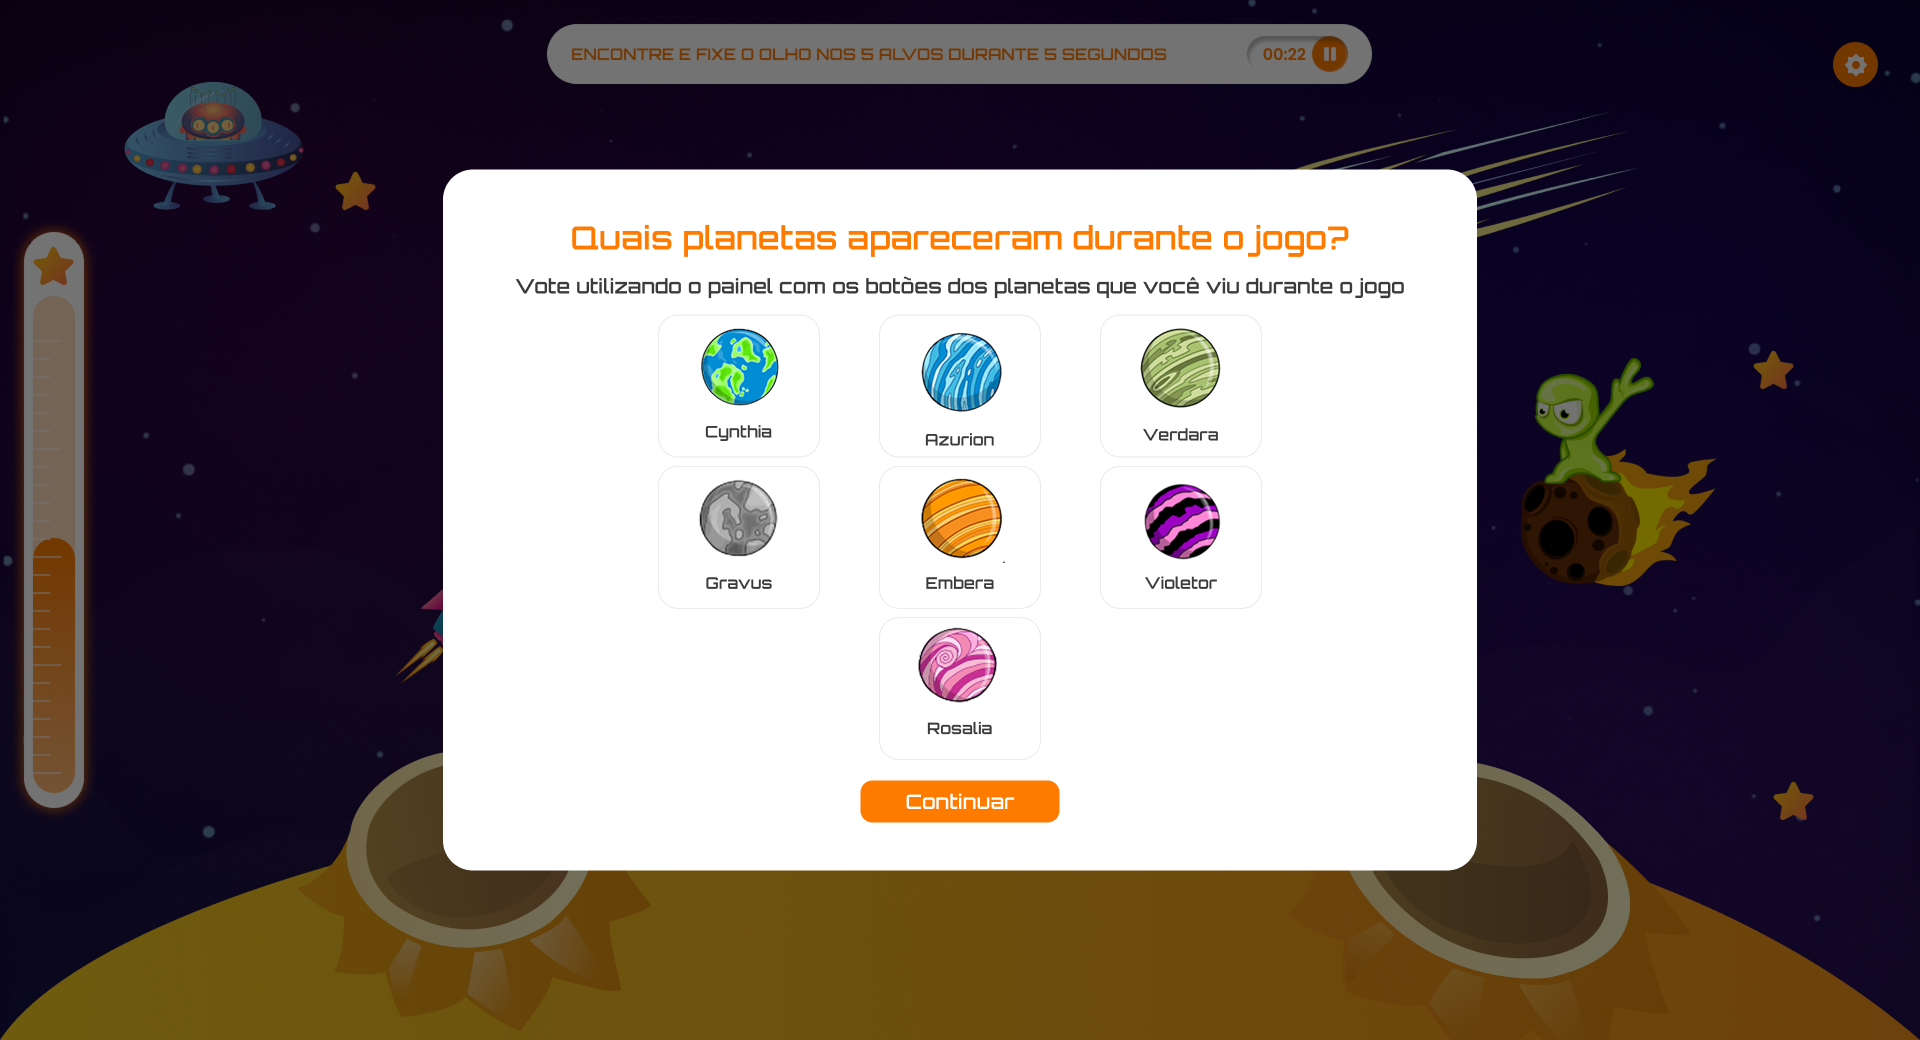
\includegraphics[width=\textwidth]{perguntas-segunda-fase.png}%
    \SourceOrNote{Autoria Própria (2025)}
\end{figure}

\begin{figure}[H]
    \centering
    \caption{Resultado da segunda fase}%
    \label{fig:fim-segunda-fase}
    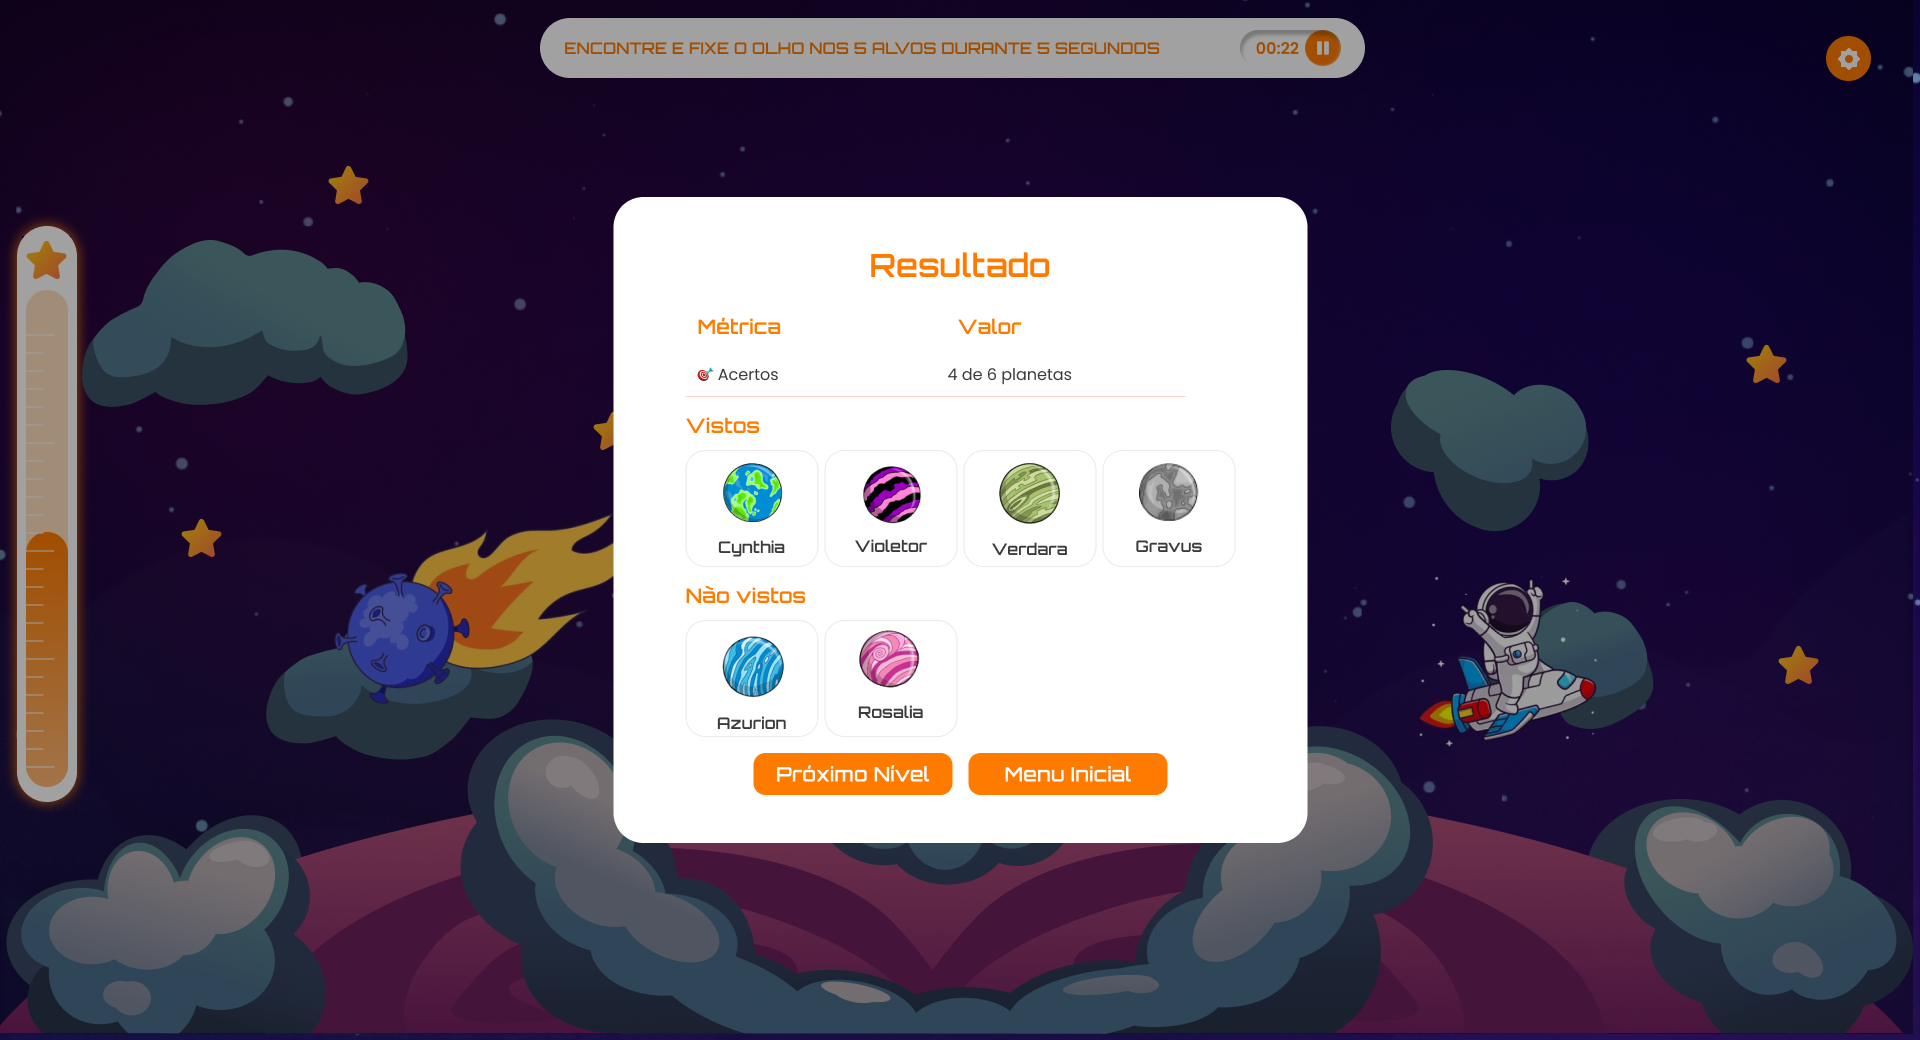
\includegraphics[width=\textwidth]{fim-segunda-fase.png}%
    \SourceOrNote{Autoria Própria (2025)}
\end{figure}

Para a construção do dispositivo de controle da \textit{IoT}, foram empregados os seguintes componentes eletrônicos: uma placa de desenvolvimento Arduino, sete botões do tipo push-button, sete resistores de 10 k$\Omega$, uma protoboard e cabos de conexão. Os botões foram conectados às portas digitais do Arduino, configuradas como entradas com resistores pull-down para garantir leituras estáveis. Dessa forma, ao término da segunda fase do jogo, o participante registra os planetas que conseguiu observar, pressionando o botão correspondente a ele. O Arduino atua como uma interface de comunicação de hardware, detectando o pressionamento físico dos botões IoT. Por meio da comunicação serial, o microcontrolador transmite o evento acionado ao sistema. O servidor é responsável por receber e interpretar este sinal do botão selecionado e, na sequência, acionar a função que contabiliza os acertos e os erros de inibição do participante para a fase.

Em futuras iterações do projeto, planeja-se o aperfeiçoamento estético e ergonômico do controle, por meio da substituição dos botões convencionais por peças personalizadas, modeladas em software CAD e fabricadas via impressão 3D, com design mais atrativo e ergonômico para crianças. Além disso, planeja-se construir uma case para o controle utilizando filamentos de garrafa PET, visando a sustentabilidade ambiental do projeto.

\begin{figure}[H]
    \centering
    \caption{Terceira fase}%
    \label{fig:terceira-fase}
    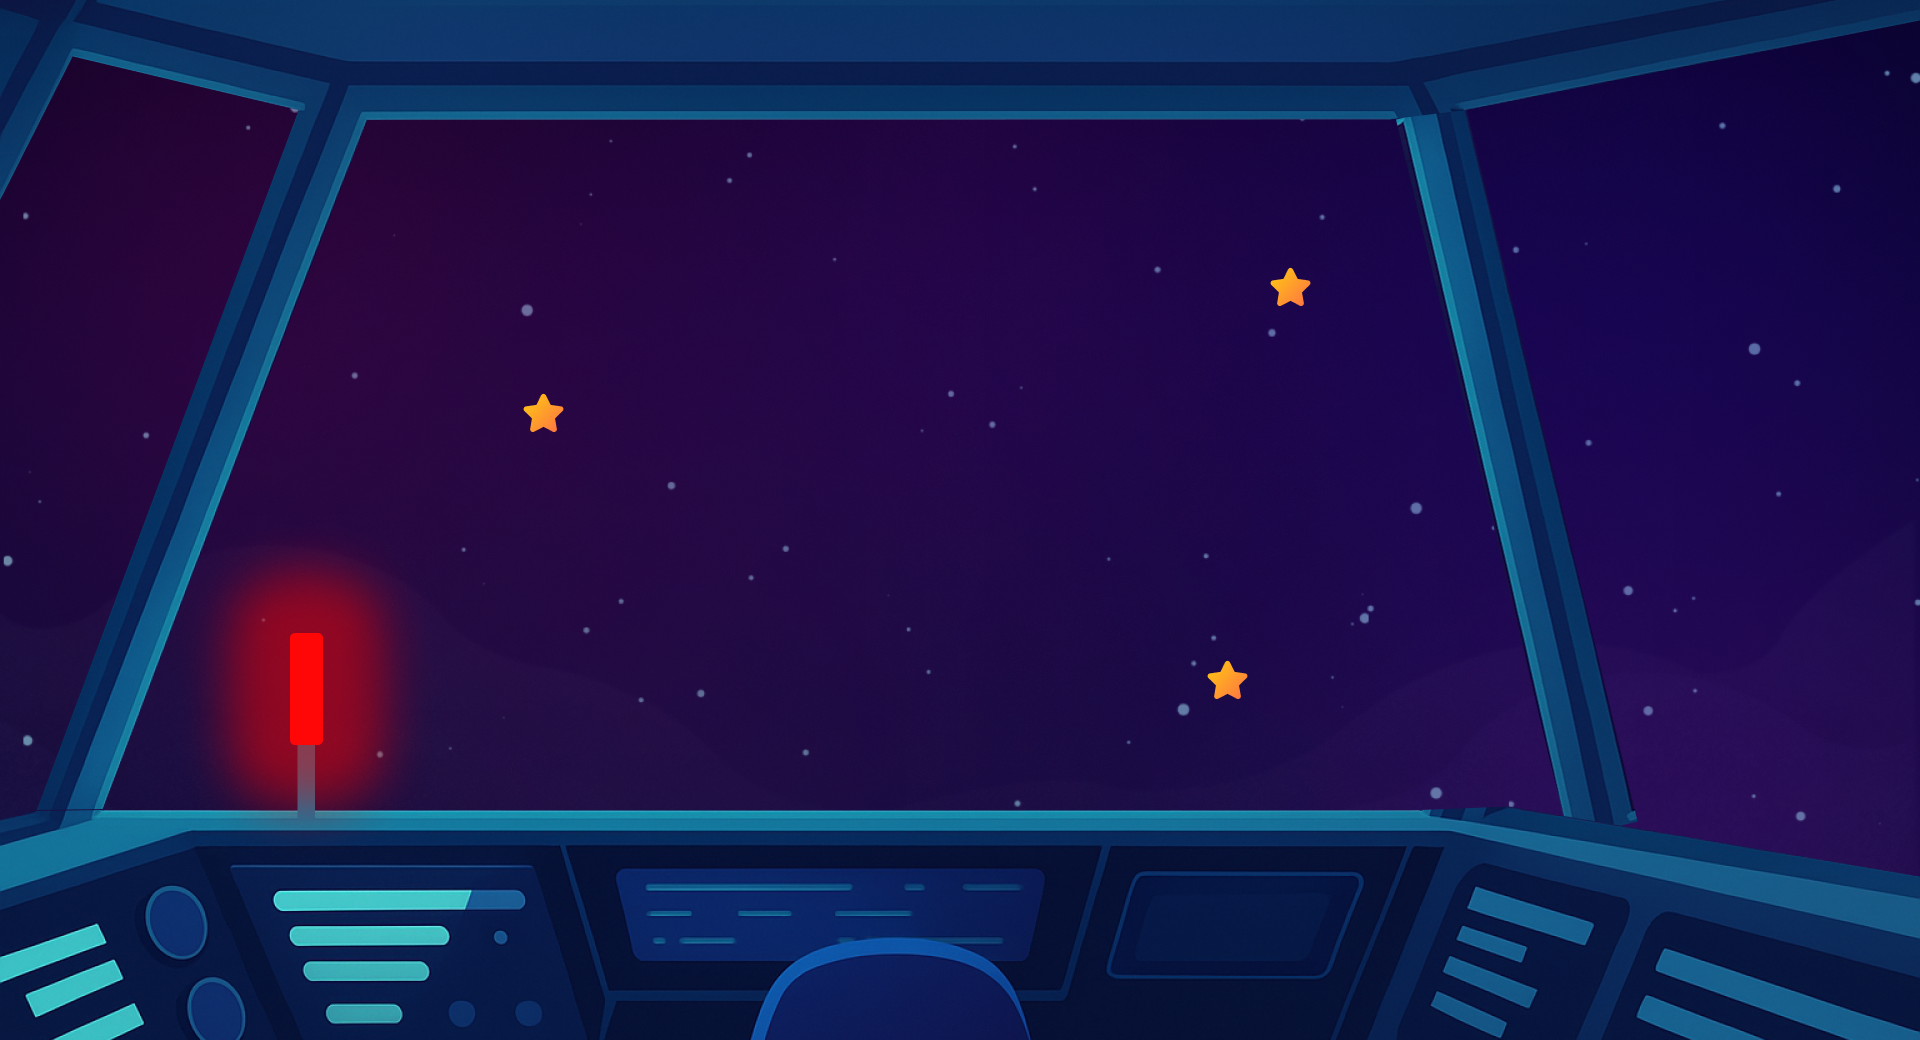
\includegraphics[width=\textwidth]{terceira-fase.png}%
    \SourceOrNote{Autoria Própria (2025)}
\end{figure}

Na terceira fase, a demanda cognitiva é intensificada pela necessidade de alternância rápida do foco visual entre diferentes regiões da tela, caracterizadas por menor previsibilidade espacial. Nessa etapa, uma estrela surge de forma estática, exigindo resposta ocular imediata do participante. Simultaneamente, um segundo estímulo estático é apresentado (radar de uma aeronave), alternando entre os estados ligado e desligado em intervalos regulares. Quando esse estímulo é ativado (ascende), o participante deve manter o olhar fixo sobre ele até que se apague, o que permite avaliar a atenção dividida e o controle do direcionamento ocular. A duração desta fase é de 30 segundos. A trilha sonora atinge seu nível máximo de intensidade e agitação, contribuindo para aumentar a complexidade da tarefa. O desempenho do participante nesta fase é utilizado como indicador da agilidade atencional e da capacidade de redirecionamento e manutenção do foco visual diante de estímulos dinâmicos.

Ao término das três fases, o sistema gera um pré-diagnóstico com base nas métricas TDC. Para isso, são utilizados os registros de desempenho e os dados mais recentes de rastreamento ocular obtidos durante as fases. Este pré-diagnóstico é elaborado por um módulo de IA, que interpreta as métricas e o desempenho do participante. O feedback resultante é apresentado em duas formas: (1) uma mensagem textual interpretativa, como: “Sua atenção está conforme o esperado”, “Sua atenção está acima do esperado” ou “Sua atenção está abaixo do esperado”, de acordo com o desempenho observado; e (2) a exibição de uma porcentagem que representa a precisão do olhar capturada pelo sistema de rastreamento ocular, conforme ilustrado na Figura \ref{fig:fim-geral}.

\begin{figure}[H]
    \centering
    \caption{Pré-diagnóstico}%
    \label{fig:fim-geral}
    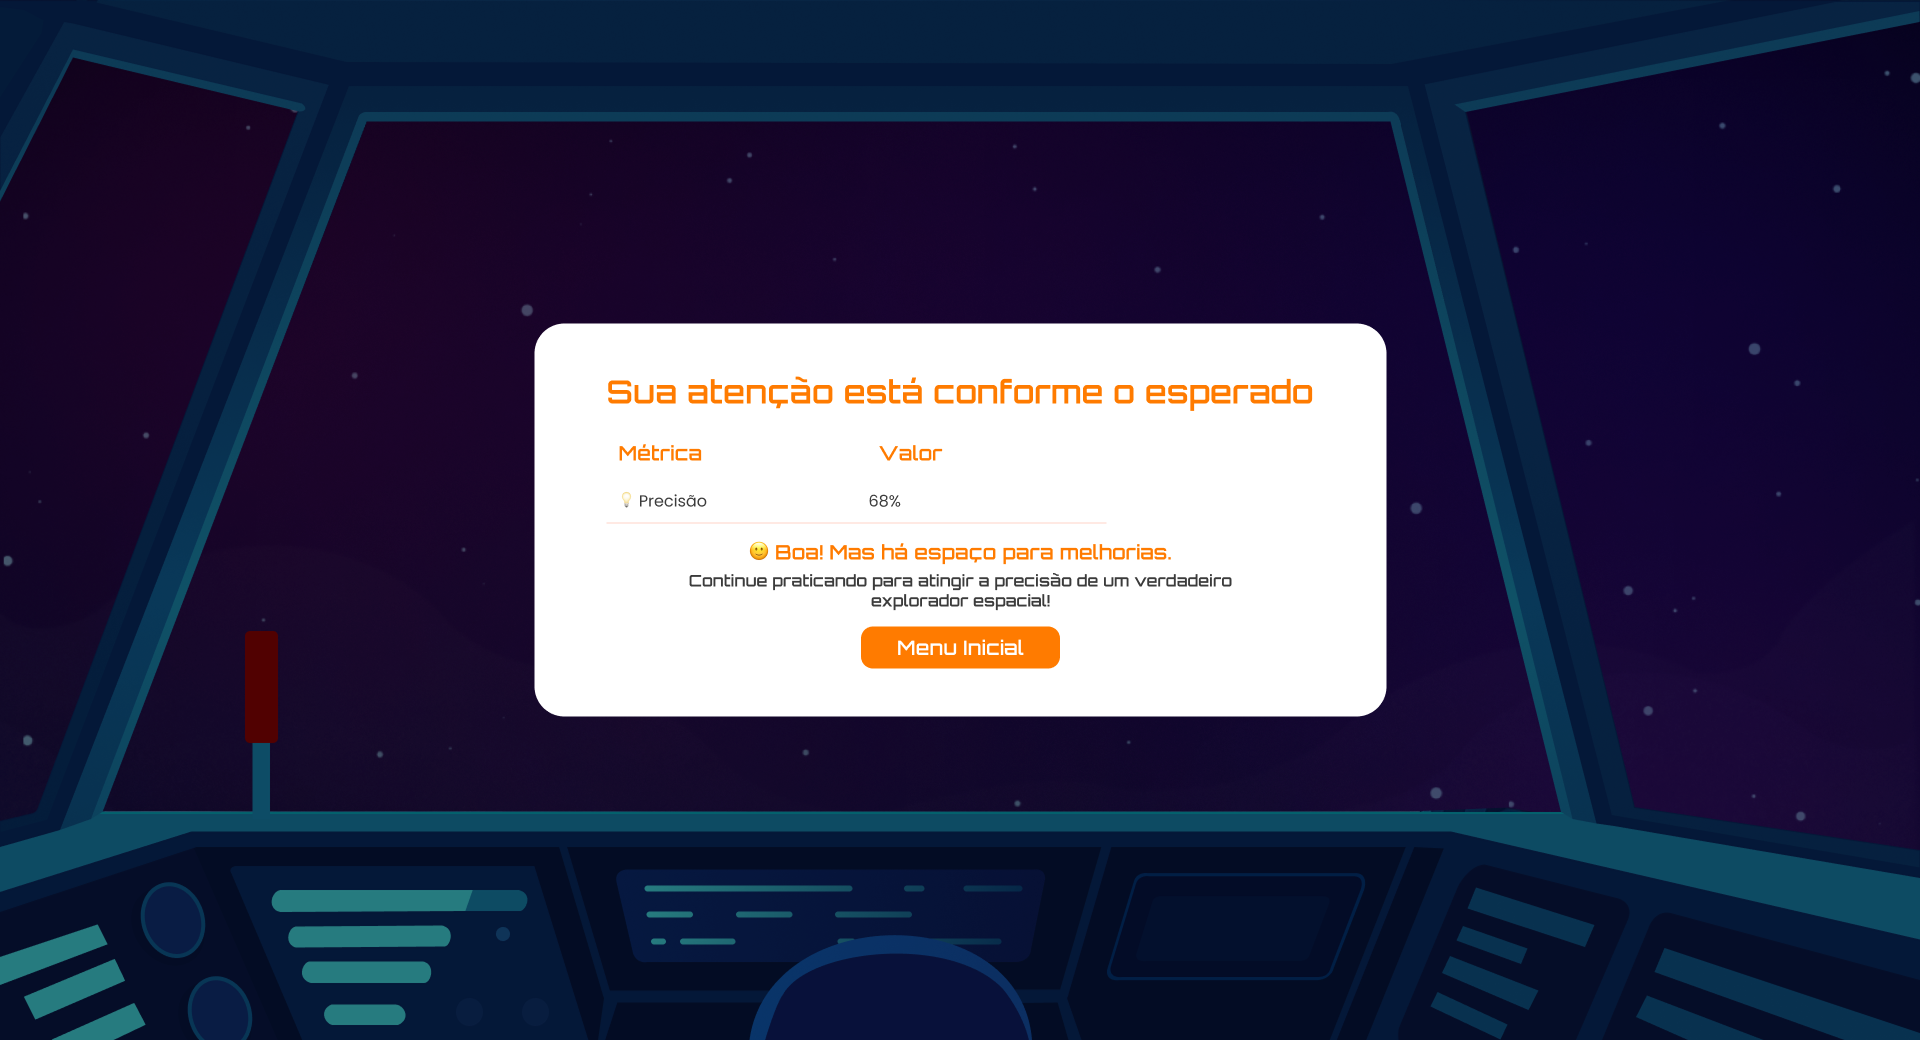
\includegraphics[width=\textwidth]{fim-geral.png}%
    \SourceOrNote{Autoria Própria (2025)}
\end{figure}

Com o objetivo de aprofundar a compreensão do tema e promover um alinhamento mais preciso entre os aspectos técnicos e psicológicos do projeto, foi conduzida uma pesquisa de campo com quatro profissionais da área da Psicologia. As entrevistas buscaram avaliar a viabilidade técnica da proposta, identificar os sintomas mais recorrentes do TDA e compreender os tipos de estímulos que mais influenciam os processos de distração em indivíduos com esse transtorno.

A análise qualitativa dos dados revelou que estímulos visuais e auditivos, especialmente movimento, cor e som, exercem papel determinante na indução de distrações, devendo, portanto, ser considerados elementos centrais no planejamento das fases experimentais. Essa lógica foi implementada em todas as fases do projeto.
Além disso, os profissionais destacaram a importância de incluir uma etapa em que os distratores estejam presentes de forma indireta, sem que o participante seja instruído a focar neles.

A plataforma é desenvolvida com tecnologias \textit{web}, permitindo acesso remoto e execução
direta em \textit{browsers} modernos. O teste é realizado de forma autônoma pelo usuário, em ambiente silencioso e seguindo instruções fornecidas pela própria plataforma.

No projeto atual, a IA será utilizada para análisar os dados coletados durante o jogo, referentes aos erros e acertos, com uma base de dados previamente formada por indivíduos diagnosticados com TDA e por outros sem o transtorno. Entretanto, nesta fase inicial de desenvolvimento, é necessário testar a viabilidade do sistema. Inicialmente, dez crianças com TDA serão convidadas a participar do experimento, com o objetivo de coletar dados iniciais que servirão como base para o treinamento supervisionado do modelo de IA. Em seguida, três crianças com TDA e três sem o transtorno (diferentes das 10 iniciais, ou seja, ainda não analisadas) 
serão convidadas para uma nova etapa experimental, destinada a validar a eficácia do sistema na identificação de indícios de desatenção. O objetivo é garantir que a acurácia do sistema seja satisfatória antes de ampliar a base de dados e aperfeiçoar o modelo de IA. Após a conclusão da fase de validação, o sistema estará apto a ser utilizado por um público mais amplo, contribuindo para a identificação precoce do TDA em crianças e reforçando seu potencial como ferramenta de apoio ao diagnóstico. 

No que se refere à retroalimentação da IA, o sistema irá conter um modo de treinamento, que pode ser ativado ou desativado exclusivamente pelo administrador. A mecânica dessa funcionalidade é empregada sempre que houver necessidade de alimentar a base de dados com novos registros. Essa etapa só pode ser executada na presença de ao menos um administrador, a fim de garantir a integridade e a qualidade dos dados inseridos. Caso contrário, a criança participa normalmente do jogo apenas para avaliar seu nível de atenção. Quando o modo de treinamento está habilitado, o sistema armazena as métricas TDC coletadas durante as partidas em uma base de dados, permitindo que o módulo de treinamento da IA realize a análise comparativa entre os dados do indivíduo e a base existente. Esse processo tem como objetivo retroalimentar o modelo e aperfeiçoar continuamente o desempenho da IA. 

Para uma melhor compreensão do funcionamento do sistema, a Figura \ref{fig:fluxograma} apresenta o fluxograma do processo, que descreve a sequência lógica das operações realizadas pelo sistema até o término das três partidas. Na etapa 1, ocorre a calibração dos olhos do jogador, processo em que o sistema identifica e ajusta os pontos de fixação ocular do usuário antes do início do jogo, garantindo a precisão do rastreamento. Em seguida, é executada a coleta das métricas TDC, que ocorre automaticamente durante as três fases do jogo. Nessa etapa, o sistema processa e registra parâmetros como número de acertos, erros de omissão, erros de comissão, tempo de reação e variabilidade temporal das respostas. Na etapa 2, há uma tomada de decisão para verificar se o participante irá jogar no modo de treinamento. Caso o modo de treinamento esteja habilitado (etapa 3), o sistema armazena as métricas TDC em uma base de dados, permitindo que o módulo de treinamento da IA realize a análise comparativa entre os dados do indivíduo e a base existente. Esse processo visa aprimorar o modelo e gerar um pré-diagnóstico personalizado. Já na etapa 4, quando o modo de treinamento não está ativado, o sistema realiza diretamente a geração e exibição do pré-diagnóstico, utilizando as métricas coletadas durante a execução do jogo.

\begin{figure}[H]
    \centering
    \caption{Fluxograma do sistema}%
    \label{fig:fluxograma}
    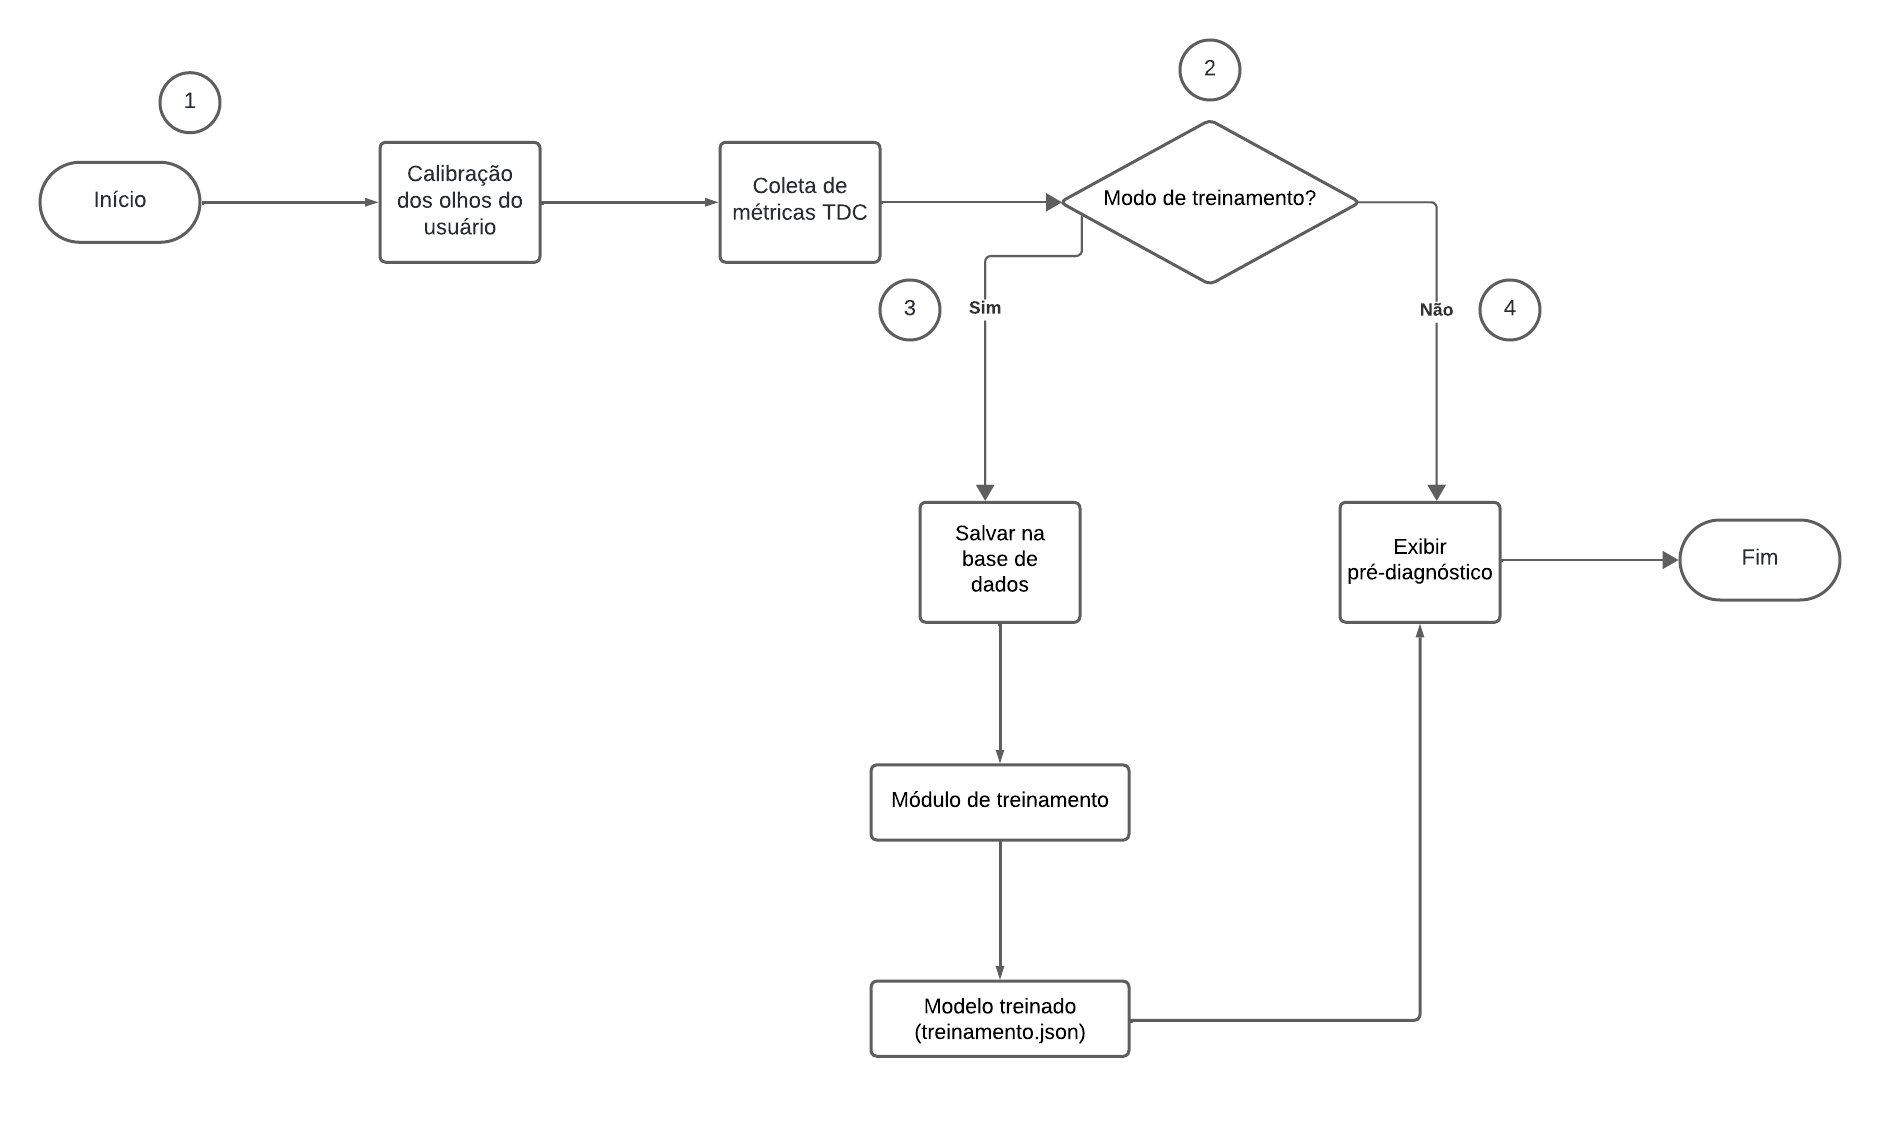
\includegraphics[width=\textwidth]{fluxograma.png}%
    \SourceOrNote{Autoria Própria (2025)}
\end{figure}

Optou-se pela utilização do banco de dados não relacional \textit{MongoDB}, o qual armazena informações em documentos no formato \textit{JSON}, possibilitando a criação de estruturas dinâmicas e aninhadas, adequadas ao armazenamento dos dados provenientes dos testes de rastreamento ocular. Sua flexibilidade e escalabilidade o tornam mais apropriado que bancos relacionais para o tratamento de grandes volumes de dados sensoriais. O gerenciamento do banco foi realizado por meio do \textit{MongoDB Compass}, ferramenta que facilita a execução de consultas, validação de esquemas e análise de desempenho.
